\documentclass[runningheads]{llncs}

%---- Sonderzeichen-------%
\usepackage[ngerman]{babel}
%---- Codierung----%
\usepackage[utf8]{inputenc}
%\usepackage[latin1]{inputenc}
\usepackage[T1]{fontenc}
\usepackage{graphicx}
\usepackage{url}
\usepackage{llncsdoc}
%----- Mathematischer Zeichenvorrat---%
\usepackage{amsmath}
\usepackage{amssymb}
\usepackage{enumerate}
% fuer die aktuelle Zeit
\usepackage{scrtime}
\usepackage{listings}
\usepackage{subfigure}
\usepackage{hyperref}

\setcounter{tocdepth}{3}
\setcounter{secnumdepth}{3}

% -------------------------------------------------------------------------------------------------
% -------------------------------------------------------------------------------------------------

\mainmatter
\title{Universal Rendering}
\titlerunning{Universal Rendering}
\author{Julian Beck}
\authorrunning{Julian Beck}
\institute{Betreuer: Prof. Dr. rer. nat. Christian Zirpins}
\date{01.05.2019}
\begin{document}
\let\oldaddcontentsline\addcontentsline
\def\addcontentsline#1#2#3{}
\maketitle
\def\addcontentsline#1#2#3{\oldaddcontentsline{#1}{#2}{#3}}

% -------------------------------------------------------------------------------------------------

\begin{abstract}
  An dieser Stelle sollte später eine Kurzzusammenfassung stehen.
\end{abstract}

% -------------------------------------------------------------------------------------------------
\tableofcontents 
\newpage
% -------------------------------------------------------------------------------------------------

\section{Einleitung}
\label{sec:Einleitung}

Seit dem Beginn des Webs funktioniert das Surfen wie folgt: 
Ein Webbrowser fordert eine bestimmte Seite an, ein Server im 
Internet bearbeitet die Anfrage und generiert ein HTML 
(Hypertext Markup Language) Dokument als Antwort. 
Dies bezeichnet man als serverseitiges rendern. 
In den Anfängen des Webs stellte dies kein Problem dar, 
da die Browser nicht leistungsstark waren und die Webseiten 
aus meist statischen Inhalt bestanden. 
Später mit HTML5 wurden Webseiten dynamischer und 
interaktiver für den Nutzer, was dazu führte, dass immer mehr Apps, 
sogenannte Single Page Applikationen, 
vollständig im Browser auf einer Seite liefen. 
Um dies zu ermöglichen wird clientseitiges rendern verwendet. 
Single Page Applications oder kurz SPAs, bieten Vorteile für den Anwender: 
Sie reagieren schnell auf Benutzerinteraktionen und können zwischen Seiten navigieren, 
ohne sie komplett neu zu laden. Gleichzeitig sind SPAs komfortabel zu entwickeln, 
dank moderner Frameworks. Beide Varianten, serverseitiges und clientseitiges rendern, 
haben Vor- und Nachteile. Universal Rendering kombiniert die beiden Ansätze und 
erfüllt alle Anforderungen an eine moderne Webanwendung.


\subsection{Anforderungen an eine Webanwendung}
\label{subsec:Anforderungen an eine Webanwendung}

Eine moderne Webanwendungen sollten folgende Anforderungen erfüllen:
\begin{itemize}
  \item Damit die Seite von Suchmaschinen gefunden werden kann, sollte sie von Suchmaschinen Crawler indexierbar sein. 
  Dies wird Suchmaschinenoptimierung oder auch SEO 
  (engl. search engine optimization) genannt. 
  \item Eine moderne Webseite muss beim Aufrufen für den Anwender schnell laden. Der Anwender sollte nicht lange warten 
  müssen bis er die Anwendung sieht und mit ihr interagieren kann
  \item Eine moderne Webanwendung muss dynamisch und interaktiv sein. Die Anwendung sollte auf Benutzereingaben reagieren, 
  ohne lange Ladezeiten oder neuladen der Seite.
  Die Anwendung sollte einfach zu entwickeln sein und gleichzeitig muss sichergestellt werden, 
  dass der Programmcode einfach zu pflegen ist. 
  Code duplikation sollte minimiert werden.
\end{itemize}

\subsection{Terminologie}
\label{subsec:Terminologie}
Beim Rendern von Webtechnologien unterscheidet man zwischen dem Rendern auf dem Server und dem Client:

\begin{itemize}
  \item SSR Server-Side Rendering: Rendern auf der Server Seite bezieht sich auf das generieren eines HTML Dokumentes 
  aus einer Single Page Application. 
  \item CSR Client-Side Rendering: Rendern auf der Client Seite bezieht sich auf das generieren und parsen eines 
  HTML Dokumentes zu einem DOM und darstellen für den Anwender. 
\end{itemize}
Der Begriff Universal Rendering beschreibt eine Kombination aus server- und clientseitiges rendern. 
Dieser Ansatz wird oft auch als Isomorphic oder Server-Side Rendering bezeichnet.
\\
\\
Folgende Begriffe beschreiben unterschiedliche Zeiten beim Laden einer Webseite:
\begin{itemize}
  \item TTFB: Time to First Byte - Zeit bis zum ersten Byte -  Die Zeit zwischen dem Klicken auf ein Link und Erhalten der Daten vom Server.
  \item FP: First Paint - der Zeitpunkt an dem der erste Inhalt für den User sichtbar wird.
  \item FCP: First Contentful Paint oder auch First Meaningful Paint - Der Zeitpunkt, an dem der Benutzer den wichtigsten Inhalt einer Website als fertig geladen sieht. Die Zeit bis zum FCP wird auch als kritischer Rendering-Pfad (engl.:Critical Rendering Path) bezeichnet.
  \item TTI: Time To Interactive - Die Zeit bis die Seite interaktiv wird und der Anwender mit ihr interagieren kann.
\end{itemize}
Da die Anwendung vollständig auf der Client Seite läuft, ist es schwierig für Suchmaschinen Crawler die seite zu Indexieren was zu einer schlechten SEO führt.
Des weiteren, dadurch dass die Webseite nicht auf dem Server, sonder vom Client gerendert wird, muss der User warten bis die seite vollständig gerendert wird.
Server Side rendering ist eine Mischung beider Ansätze. Es kombiniert die SEO und Performance von Server seitigen Applikationen und die Interaktivität und flexibilität von Client Side Anwendungen.
\\
\\
Diese Arbeit beginnt mit den der Funktionsweise von server - und clientseitigen Rendern. Es werden die Vor - und Nachteile der jeweiligen Vorgehensweisen untersucht und beschrieben warum eine Notwendigkeit für Universal Rendering besteht. Nach einer Einführung in den Universal Rendering Vorgang, werden die verwendeten Technologien und deren Funktionsweise für das Rendern beschrieben. Anschließend werden die positiven und negativen Aspekte des Universal Rendering beschrieben und Alternativen genannt. Danach beschreibt die Arbeit unterschiedliche Frameworks zum implementieren der Rendering Technologie und zeigt wie Unternehmen Universal Rendering verwenden. Das Fazit erarbeitet wann welche Rendering Technologie verwendet werden soll und zeigt den aktuellen Stand von Suchmaschinen Crawler.

% -------------------------------------------------------------------------------------------------

\section{Serverseitiges Rendering}
\label{sec:Serverseitiges Rendering}

\begin{figure}[h]
  \centering
  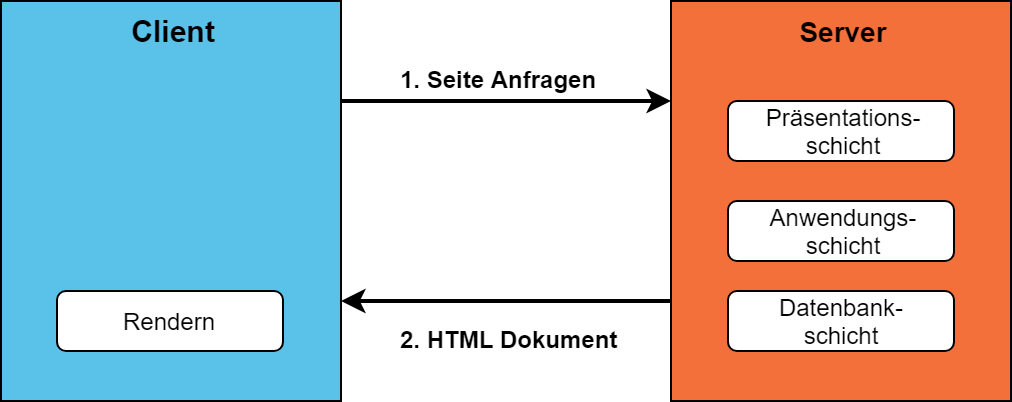
\includegraphics[width=12cm]{images/server}
  \caption{HTMl Dokument einer React Seite}
\end{figure}



\subsection{Serverseitiges Rendering mit Ajax}
\label{subsec:Serverseitiges Rendering mit Ajax}

\begin{figure}[h]
  \centering
  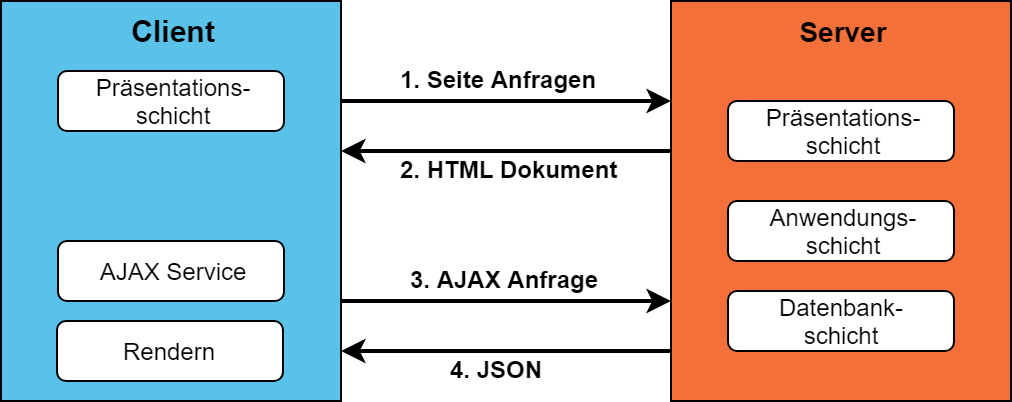
\includegraphics[width=12cm]{images/serverajax}
  \caption{HTMl Dokument einer React Seite}
\end{figure}


Dies ist ein Zitat \cite{becker2008a}.
test\cite{IsomorphicApps}
test\cite{SearchFriendly}
test\cite{chen_chen_2016}

\newpage
% -------------------------------------------------------------------------------------------------

\section{Clientseitiges Rendering}
\label{sec:Clientseitiges Rendering}

\begin{figure}[h]
  \centering
  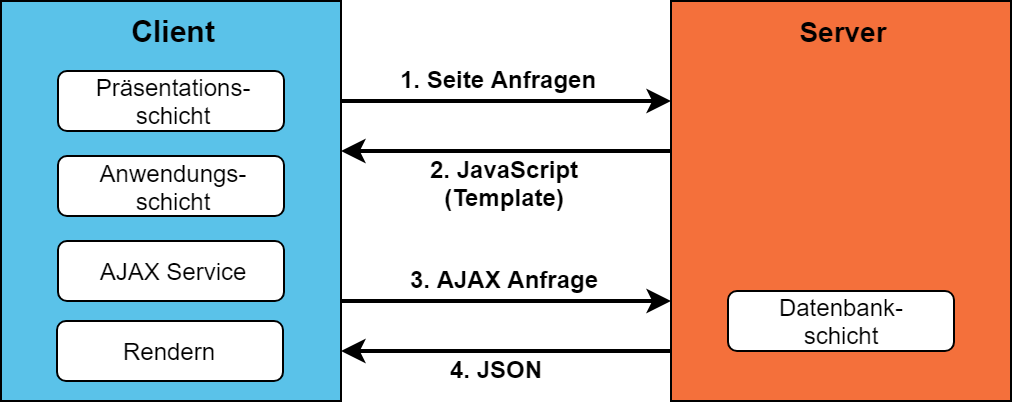
\includegraphics[width=12cm]{images/client}
  \caption{HTMl Dokument einer React Seite}
\end{figure}

\begin{figure}[h]
  \centering
  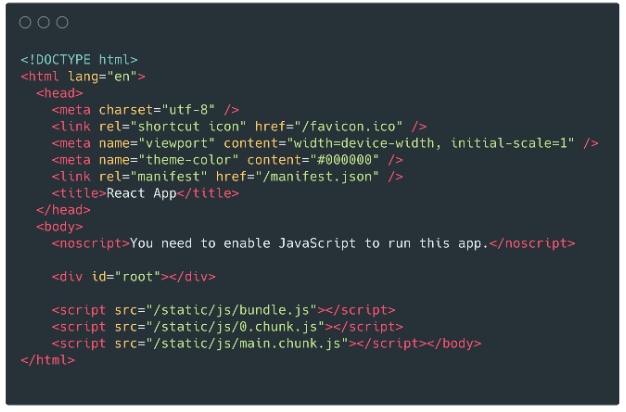
\includegraphics[width=9cm]{images/react-code-small}
  \caption{HTMl Dokument einer React Seite}
\end{figure}


\newpage
% -------------------------------------------------------------------------------------------------

\section{Universal Rendering}
\label{sec:Universal Rendering}

\begin{figure}[h]
  \centering
  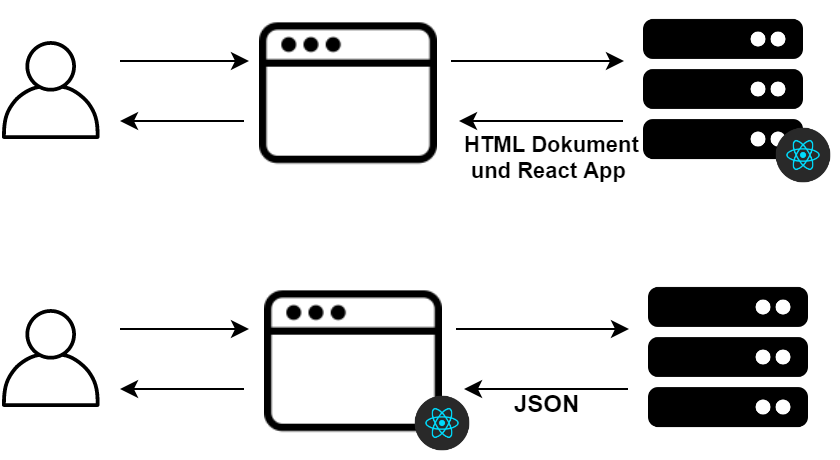
\includegraphics[width=12cm]{images/react}
  \caption{HTMl Dokument einer React Seite}
\end{figure}


\begin{figure}[h]
  \centering
  
\includegraphics[width=10cm]{images/universalseo}
  \caption{HTMl Dokument einer React Seite}
\end{figure}

\subsection{Isomorphic JavaScript}
\label{subsec:Isomorphic JavaScript}

\subsection{Virtuelles DOM}
\label{subsec:Virtuelles DOM}

\begin{figure}[h]
  \centering
  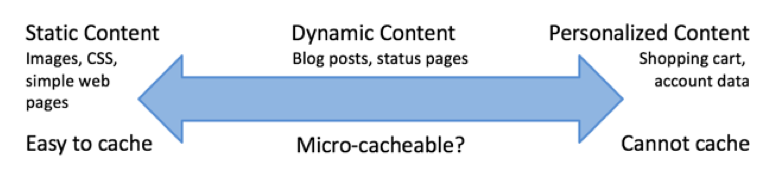
\includegraphics[width=5cm]{images/caching}
  \caption{HTMl Dokument einer React Seite}
\end{figure}

\subsection{Clientseitige Hydration}
\label{subsec:Clientseitige Hydration}

\begin{figure}[h]
  \centering
  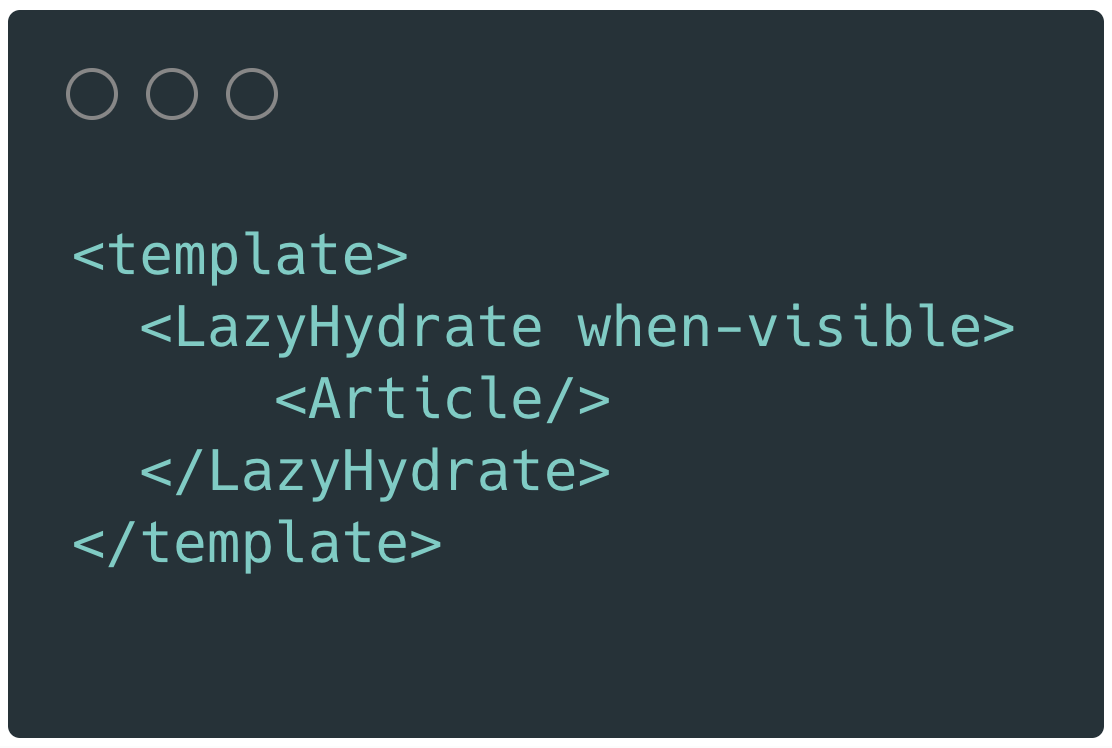
\includegraphics[width=5cm]{images/LazyHydration}
  \caption{HTMl Dokument einer React Seite}
\end{figure}

\subsection{Rendering Ablauf}
\label{subsec:Rendering Ablauf}

\begin{figure}[h]
  \centering
  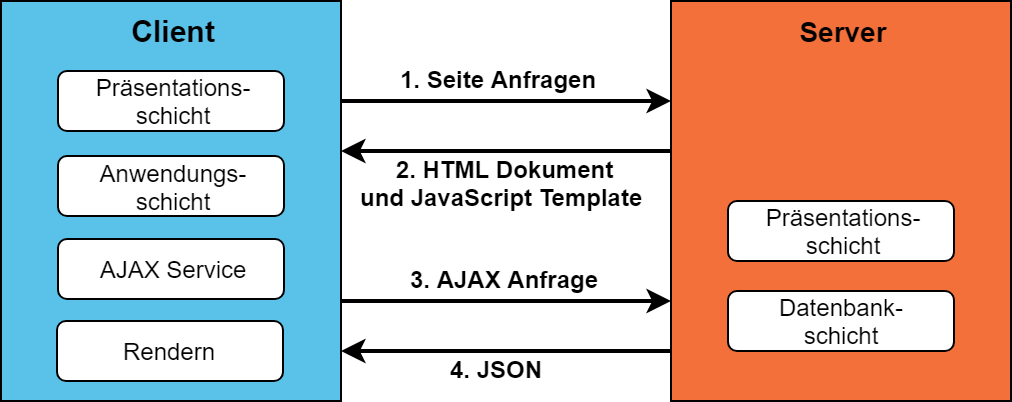
\includegraphics[width=12cm]{images/universal}
  \caption{HTMl Dokument einer React Seite}
\end{figure}

\newpage
\subsection{Vorteile}
\label{subsec:Vorteile}

\begin{figure}[h]
  \centering
  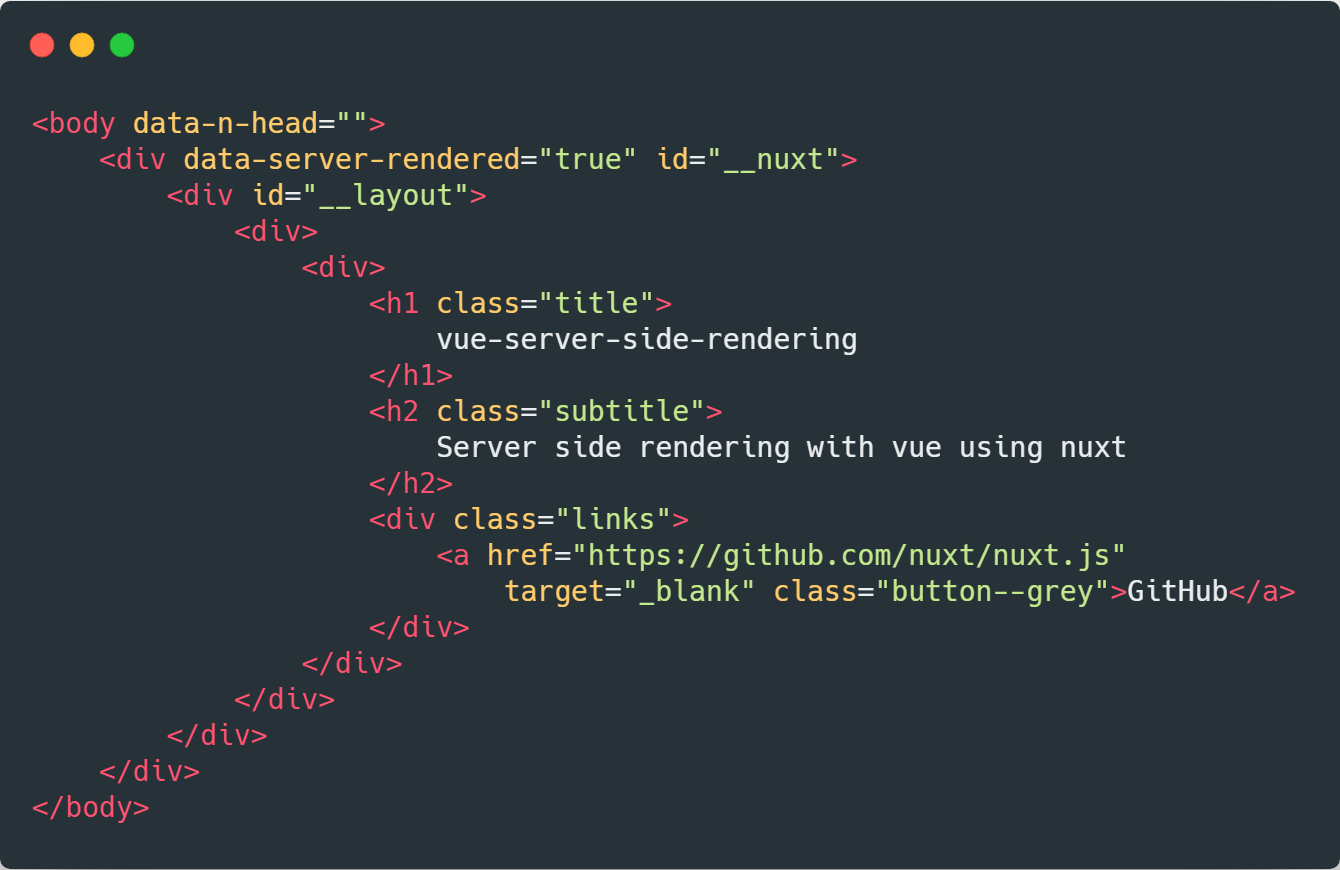
\includegraphics[width=9cm]{images/nuxt-body-first}
  \caption{HTMl Dokument einer React Seite}
\end{figure}

\subsection{Nachteile}
\label{subsec:Nachteile}

\subsection{Alternativen}
\label{subsec:Alternativen}

\begin{figure}[h]
  \centering
  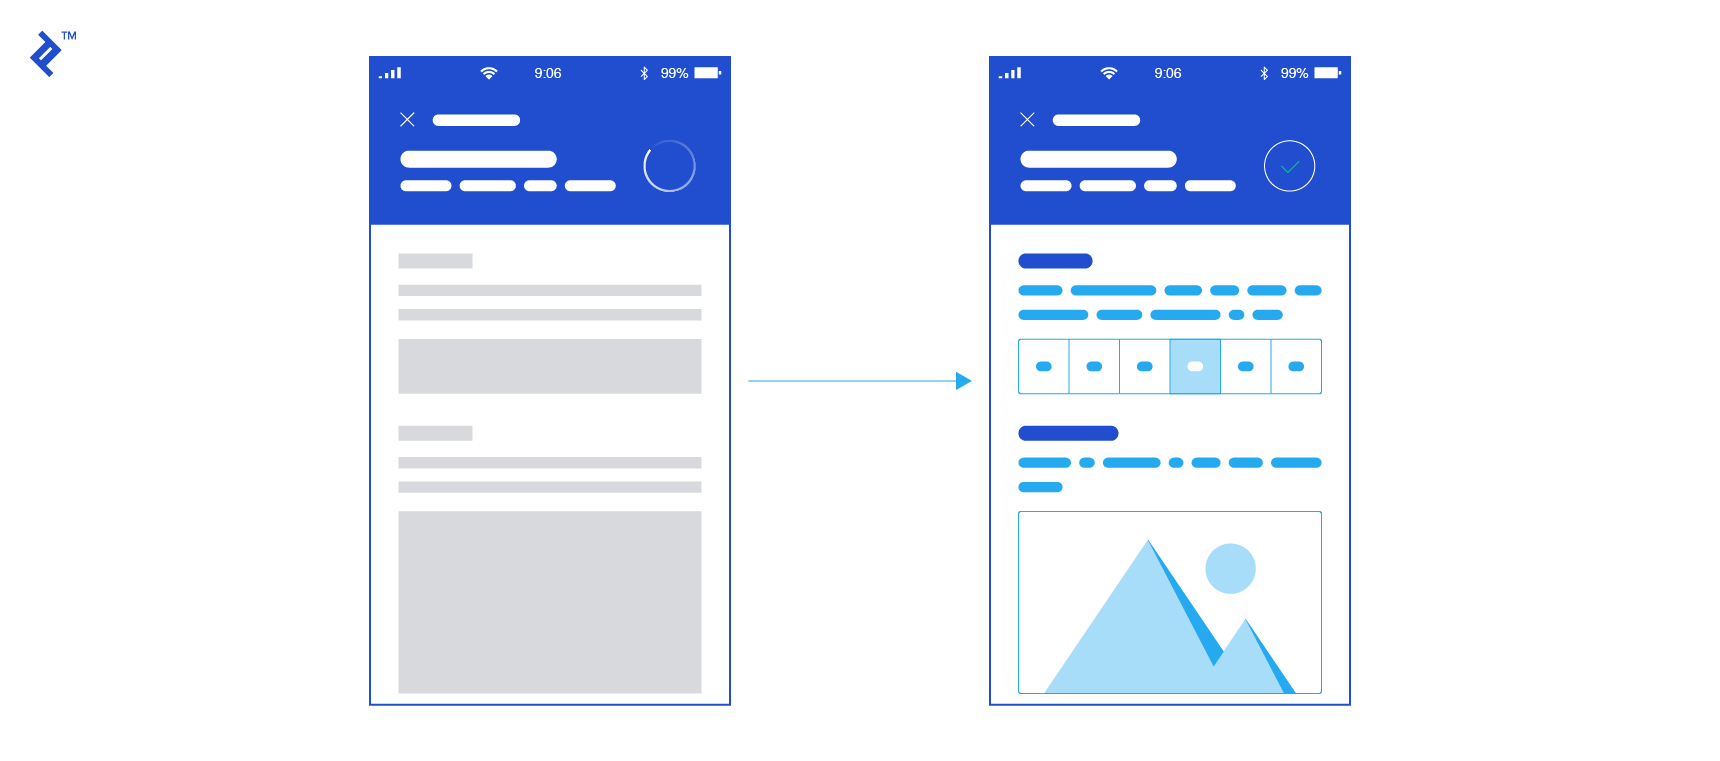
\includegraphics[width=9cm]{images/WebsiteSceleton}
  \caption{HTMl Dokument einer React Seite}
\end{figure}

\newpage
% -------------------------------------------------------------------------------------------------

\section{Frameworks}
\label{sec:Evaluation}

\subsection{React und Next.js}
\label{subsec:React und Next.js}

\begin{figure}
  \centering
  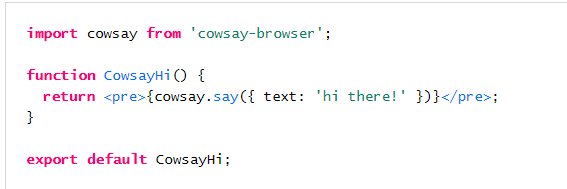
\includegraphics[width=10cm]{images/CodeSplitting}
  \caption{HTMl Dokument einer React Seite}
\end{figure}

\begin{figure}
  \centering
  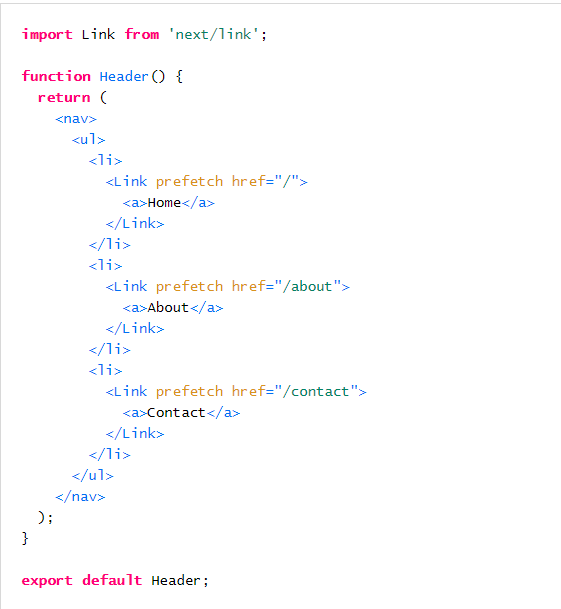
\includegraphics[width=7cm]{images/prefetchnext}
  \caption{HTMl Dokument einer React Seite}
\end{figure}


\subsection{Vue.js und Nuxt.js}
\label{subsec:Vue.js und Nuxt.js}

\subsection{Angular Universal}
\label{subsec:Angular Universal}

\newpage
% -------------------------------------------------------------------------------------------------

\section{Universal Rendering in der Praxis}
\label{sec:Universal Rendering in der Praxis}

\newpage
% -------------------------------------------------------------------------------------------------

\section{Fazit und Ausblick}
\label{sec:Fazit}

\begin{figure}
  \centering
  
\includegraphics[width=10cm]{images/HackerNews}
  \caption{HTMl Dokument einer React Seite}
\end{figure}

\begin{figure}
  \centering
  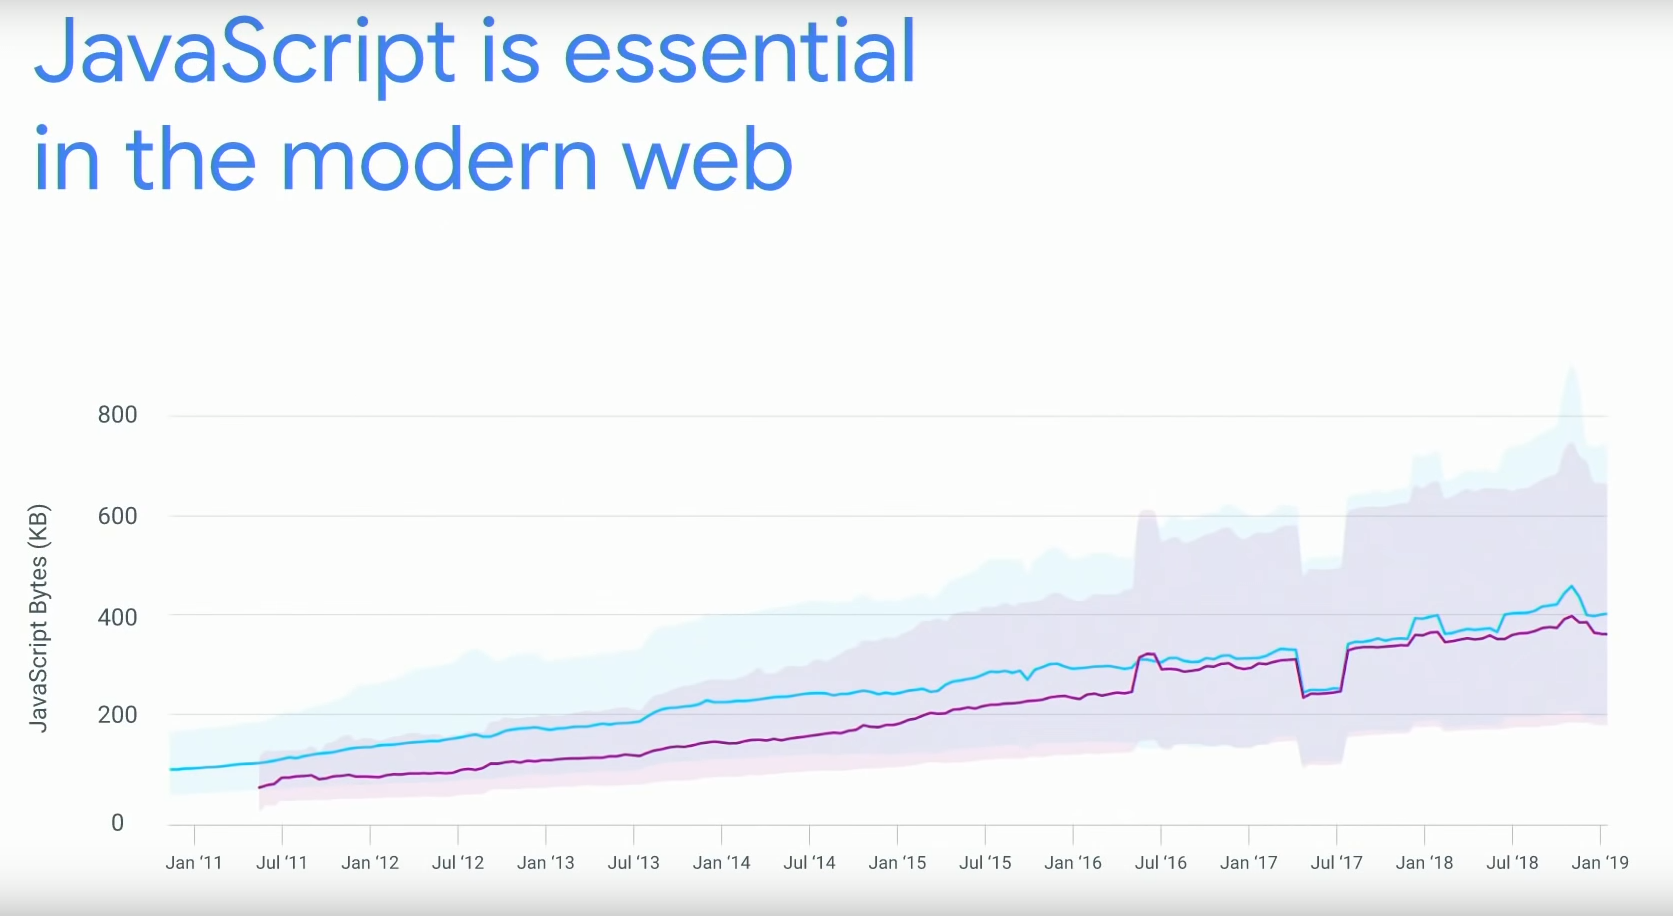
\includegraphics[width=10cm]{images/JavaScriptGoogleShips}
  \caption{HTMl Dokument einer React Seite}
\end{figure}




% -------------------------------------------------------------------------------------------------
\newpage
% Normaler LNCS Zitierstil
%\bibliographystyle{splncs}
\bibliographystyle{itmalpha}
% TODO: Ändern der folgenden Zeile, damit die .bib-Datei gefunden wird
\bibliography{literatur}

\end{document}
